%!TEX TS-program = pdflatex
%!TEX root = i3det-top.tex
%!TEX encoding = UTF-8 Unicode

\section{Drilling and Deployment}

\subsection{Hot Water Drilling}

IceCube transformed a cubic kilometer of Antarctic ice into an astrophysical particle detector composed of 86 cables (strings) of DOMs buried deep beneath the surface.  Each string required drilling a borehole approximately 60 cm in diameter to a depth of 2,500 m.  The 5 MW Enhanced Hot Water Drill (EHWD) was designed and built specifically for this task, capable of producing the required boreholes at a rate of one hole per 48 hours. Hot water drilling on this scale presented unique challenges that were successfully met with the EHWD.

Large-access holes were required at a high production rate.  Hot water drilling was selected as the best method due to its inherent speed.  Indeed, hot water drilling is the only feasible technology to provide rapid access to the deep ice on this scale.  Additionally, leaving the boreholes water-filled during drilling allowed for the deployed instrumentation to become frozen in place and optically coupled with the surrounding ice sheet.
 
Hot water drilling in this case involved a drilling phase to create the initial hole, followed by an upward reaming phase to give the hole a targeted diameter profile.  Hole diameter was oversized to compensate for closure from freezeback to provide sufficient time to deploy instrumentation, with contingency time for delays.  The elapsed duration from the end of drilling until the hole closes to below specification is referred to as the hole lifetime.  Substantial resources were invested in modeling the thermodynamics and shape of the hole over time to optimize hole lifetime and fuel consumption (Greenler, in press).

The Enhanced Hot Water Drill was designed and built to accomplish this task, and was continually refined over the course of IceCube construction.  At the project’s end, the EHWD had drilled 86 holes, each nominally 60 cm in diameter and 2,500 m deep, in seven field seasons (approximately 21 months total time).  Peak performance occurred in the 2009-2010 season with 20 holes drilled (early November to mid-January).  

The highest-level EHWD system design requirements were to:

\begin{enumerate}
\item	Deliver 80 boreholes, each 60 cm diameter and 2,500 m deep (actually delivered 86 holes),
\item	complete drilling and instrumentation deployment in seven field seasons (2004-2011),
\item	withstand the South Pole environment (average austral summer temperature -33$^{\circ}$ C, winter storage minimum temperature -80$^{\circ}$ C, altitude approximately 3,000 m),
\item	stay compatible with South Pole logistics (all large cargo and fuel transported by LC-130 aircraft),
\item	simultaneously support deployment of in-ice instrumentation (to streamline the drilling-deployment flow),
\item	minimize drill time and fuel consumption, and
\item	maintain safe and predictable operations.
\end{enumerate}

The design philosophy for the EHWD was to leverage and build upon the drilling experiences of AMANDA (Antarctic Muon and Neutrino Detector Array – Koci, 1994; AMANDA Collaboration, 2001; Koci, 2002), the prototype detector that served as a proof of principal for IceCube.  This was accomplished by reusing equipment where appropriate, recruiting expertise, and incorporating the following major enhancements:

\begin{enumerate}
\item	Doubled thermal capacity (2.3 MW to 4.7 MW),
\item	continuous drill hose on a single hose reel (eliminating the need to add/remove hose segments throughout drilling/reaming),
\item	extensive system automation,
\item	two drilling structures (allowing for streamlined drilling-deployment flow),
\item	modular design,
\item	high-efficiency water heaters (to reduce fuel consumption), and
\item	improved drilling strategy (optimizing hole shape to avoid over-drilling the borehole diameter and wasting fuel).
\end{enumerate}

The EHWD system was implemented across two separate sites.  The seasonal equipment site (SES) provided electricity and a stable supply of hot pressurized water, and the tower operations site (TOS) was where the hole was drilled.  The two sites were linked by long cables and insulated hoses.

The SES was comprised of generators, water tanks, pump and heating buildings, a central control building, mechanical and electrical shops, spare parts storage, and system Rodwell.  All of the equipment was packaged into customized ISO shipping containers that fit into an LC-130 aircraft and tailored to its specific building functions.  These packaged containers were called mobile drilling structures (MDS).  Hoses and cables connected SES subsystem buildings together, and wherever possible custom electrically heated hoses were installed, providing an effective freeze mitigation strategy.

The TOS included the drill tower and attached operations building as well as the hose and cable reels.  There were two towers and one set of drill reels.  After drilling, drill reels were moved to the next hole location, where the second tower had already been staged.  The first tower stayed at its existing location to support deployment of the instrumentation.  Once deployment had finished, the first tower could be moved to the next location while drilling at the second tower was underway.  This leapfrog sequence of the tower structures reduced hole turnover time and allowed for nearly continuous drilling operations.

Due to the massive size and complexity of the SES, it remained stationary throughout each drill season.  At the end of the drill season, the SES was decommissioned and repositioned within a virgin sector of the IceCube array, staged for the following drilling season.  The distance between the SES and TOS had a practical limit, referred to as reach, which defined the boundary of a seasonal drilling sector.  Reach of the EHWD was 450 m, limited by pressure and voltage drop through the SES-TOS link.  During the last two seasons of IceCube construction the SES supported two drilling sectors from the same SES location, demonstrating a reach of 430 m.

Each drilling season started with a staggered arrival of drill crew members while the SES and TOS were excavated and commissioned.  Season startup tasks included SES and TOS warming and hookups, reinstallation of do-not-freeze equipment (such as motor drives, sensors, and some rubber/gaskets), generator commissioning, safety checkout and system tuning, seed water delivery, and Rodwell development.  This phase typically took four weeks, three of which had a full crew of approximately 30 drillers.  Once seed water was delivered, the transition was made to around-the-clock operations spread across three 9-hour shifts.

The production drilling sequence was to drill, ream, and move to the next location.  Independent firn drilling stayed ahead of deep drilling by no fewer than a couple of holes, and often the Rodwell and first few holes of the season had already been firn-drilled the prior season.  The phase between holes, called idle, was characterized by minimal flow through the system and fine-tuning of Rodwell management strategies.  The idle phase also included regular maintenance tasks and deployment of IceCube instrumentation.  Hole production rate was 48 hours per hole on average, and the quickest cycle time was 32 hours.

System shutdown would begin approximately two weeks before season’s end.  Shut down tasks included flushing the system with propylene glycol, blowing out the plumbing with compressed air, removing do-not-freeze equipment for warm storage, storing the TOS structures and other support equipment, and finally moving the SES into location for the following season.

During steady drilling operations, a minimum of four people were needed to operate the drill (drill control center, SES float, TOS control, TOS float), but a full shift was required to move hole locations and aid in deployment.  Minimum shift size was nine team members – this allowed for one sick worker and a 4/4 split lunch.  A critical part of the staffing plan was to have a good spread of expertise on all shifts, including a shift lead and deputy lead comfortable with all aspects of the system and its operation, a safety officer (duty of the deputy lead), an electronics expert, a heater expert, a software expert, and mechanically proficient technicians.  The most important thing IceCube did to assure successful drilling operations was put a strong focus on retention of experienced drillers and talent.

A strong safety culture was an essential aspect of drilling and deployment operations.  Annually-reviewed safety processes included a safety manual, 34 standard operating procedures, 18 hazard analyses, and a series of checklists.  In the field, safety briefs, emergency management exercises, near-miss incident reporting, and peer safety audits became matter of course.  Off the ice, a 2-week driller training course was organized each year to highlight system technical updates, discuss plans for the coming season, and provide further safety and first aid training.  As a result of this safety culture, IceCube had only 4 lost time drilling-related safety incidents in approximately 52 on-ice person-years.

\vspace{\baselineskip}

\begin{minipage}{\textwidth}
  \centering
\captionof{table}{EHWD System Characteristics}
  \begin{tabular}{ l | r }
    \bf{Specification} & Value \\
    \hline	
    Total Power (Thermal + Electrical) & 5 (4.7 + 0.3) MW \\
    Maximum Drill Speed & 2.2 m/min \\   
    Maximum Ream Speed & 10 m/min \\
    Water Flow (delivered to main hose) & 760 l/min \\
    Water Temperature (delivered to main hose) & \SI{88}{\celsius} \\
    Water Gauge Pressure (at main pumps) & 7,600 kPa\\
  \end{tabular} 
  \label{tab:ehwd_system}
\end{minipage}
\vspace{\baselineskip}
%\begin{minipage}{6cm}
%  \centering
%  \begin{tabular}{ l | r }
%    \bf{Specification} & Value \\
%    \hline	
%   Total Fuel\footnote{\label{note1}Total Fuel includes deep drilling/reaming and firn drilling}, AN-8 & 21,000 L \\
%    Time to Drill/Ream & 30 hr \\   
%    Hole Production Cycle Time\footnote{\label{note2}Hole Production Cycle Time is the elapsed time from start of one hole to start of the next hole} & 48 hr \\
%  \end{tabular}
%  \captionof{table}{Average performance for 24-hour lifetime hole of 2500 m depth} 
%  \label{tab:ehwd_system_avg}

\begin{minipage}{\textwidth}
  \centering
  \captionof{table}{Average and peak performance for a 24-hour lifetime hole of 2500 m depth. (Peak taken from IceCube hole 32)}
  \begin{tabular}{ l | r  | r }
    \bf{Specification} & Avg Value  & Peak Value\\
    \hline	
    Total Fuel\footnote{Total Fuel includes deep drilling/reaming and firn drilling}, AN-8 & 21,000 L & 15,000 L \\
    Time to Drill/Ream & 30 hr& 27 hr \\   
    Hole Production Cycle Time\footnote{Hole Production Cycle Time is the elapsed time from start of one hole to start of the next hole} & 48 hr & 32 hr \\
    \end{tabular}
  
  \label{tab:ehwd_system_peak}
\end{minipage}
\vspace{\baselineskip}

%\begin{enumerate}
%\item	Hole diameter remains greater than 45 cm for 24 hours after completion of drilling.
%\item	Total Fuel includes deep drilling/reaming and firn drilling.
%\item	Hole Production Cycle Time is the elapsed time from start of one hole to start of the next hole.
%\item	IceCube hole 32.
%\end{enumerate}

With the EHWD, we have demonstrated that is it possible to do large-scale production ice drilling in the Antarctic environment in a safe, efficient, and predictable way.  Critical components of IceCube’s successful drilling campaign included a large engineering investment, steadfast year-to-year support to properly address lessons learned, a strong safety culture, and priority on retention of experienced crew members.

\subsection{Deployment and Deployment instrumentation}

DOM deployment required 60 DOMs staged in the drill tower, various attachment hardware, pressure sensors and the downhole cable that was setup on a spool outside the drill tower. After verification that the hole was ready for deployment and a pre-deployment safety check, the downhole cable was pulled over the tower crescent above the open hole. Four 100 pound weights were connected together and attached via a 2.1m steel cable to a DOM that had a 17 meter (long) penetrator assembly. The weights and lowermost DOM were attached to the bottom of the downhole cable via a 15.5m steel cable. After lowering of the DOM and weights, the next DOM with a 1.8M penetrator assembly was attached to the downhole cable. The 2 DOMs were then electrically connected to the downhole cable at the breakout assembly. A Paro Scientific pressure sensor was attached just above the 2nd DOM. The pressure sensor was readout during deployment to confirm that the string was indeed dropping into the hole and not getting stuck. Alternatively, DOMs with 17m and 1.8m penetrator assemblies were attached to the downhole cable. This was continued until 60 DOMs were attached to the downhole cable at 30 breakouts. Once all the DOMs were attached, the remaining 1.5km of downhole cable was lowered into the hole. The top of the cable was secured by a large 8x8 inch deadman trenched into the snow near the hole. After the cable was secure, it was taken off of the spool and connected to the Surface Junction Box.

\subsection{Geometry Calibration}

The geometry of the detector is determined using drill and survey data
during deployment (stage 1), and then corrected and refined using the LED
flashers in ice (stage 2).
\subsubsection{Stage 1 Geometry Calibration}
The (x,y) coordinates of the string are calculated using the position
of the drill tower. Before deployment, when the drill tower is in position, at least three
of the tower corners are surveyed from at least one control point.
The coordinates for the center of the hole in the tower floor are
calculated from the corner coordinates. If x-y drift vs. depth has been calculated for the hole from drill
data, the drifts are added to the (x,y) coordinates of individual
DOMs, assuming that the string follows the hole center.

The depth of the lowest DOM on the string is calculated using pressure
readings from the Paro/Keller pressure sensor, converted to depth by correcting
for the compressibility of the water in the hole and the ambient (air)
pressure measured before the pressure sensor hits the water. The
distance from the tower floor to the water surface is measured with a
laser ranger. The vertical DOM spacings are also measured with a laser
ranger.

\subsubsection{Stage 2 Geometry Calibration}


The LED flashers are used to correct the relative depths of the
strings. This correction is typically less than 1~m relative to the
stage 1 data, but can be as large as 20~m (larger than the 17~m DOM
spacing) in cases where the pressure sensor fails during string
deployment before it takes the final depth reading. The correction is
calculated by finding the leading edge of the time distribution of the
light recorded by the
receiving DOM, denoted $t_0$. The distance corresponding to the
leading edge time is $d = c_{ice} \cdot t_0$, and the distances for
all receiving DOMs are plotted as a function of the vertical distance
between the flasher and the receiver, $z' = z_{receiver} -
z_{flasher}$. The resulting plot described a hyperbola, $d = \sqrt{D^2
+ (z' -\Delta z)^2}$, where $D$ is the horizontal distance between the
flasher string and the receiver string, calculated from stage~1 data,
and $\Delta z$ is the relative offset between the depths of the
flashing and receiving string. The hyperbola fit is done
simultaneously for each flashing string and all surrounding receiving
strings in order to calculate the relative offsets, which are then
applied to the z coordinate of all DOMs on the string.

{\it Trilateration}

Flasher corrections to the (x,y) coordinates of some DOMs in the
center of the DeepCore subarray were calculated using the
trilateration method. In this analysis, the 5~DOMs closest to the
flasher on each of the three closest strings surrounding the flasher are selected,
and a circle of radius $r = \sqrt{(d)^2 - (\Delta z)^2)}$ is drawn
around each receiving DOM, where $d$ is the distance between the DOM and the flasher calculated from the leading edge time of the received
light, and  $\Delta z$ is the relative depth of the flashing and
receiving DOMs calculated from the method described above. The
intersection points of all the circles are calculated, and the (x,y)
position of the flashing DOM is taken to be the average of the
centroid of the intersection points. The error bars on the positions
are $1 \sigma$ from a Gaussian fit to all centroid values; the x and y
corrdinates are fitted independently. The shifts relative to the
deployment data are found to be less than 1~m, and agree with the
drill head coordinates within the error bars.

\subsubsection{Inclinometers}

The stability of the East Antarctic ice sheet is one key feature making it suitable for a particle physics installation.  However, glaciers will deform mechanically under the stress of their own weight.  IceCube installed $\sim$50 inclinometers in the deeper sections of the array:  three electrolytic inclinometers (Applied Geomechanics Inc., Santa Cruz, CA) housed in $\sim$20-cm-long aluminum pressure modules were installed during the 2007-08 season and 48 micro-electromechanical (MEMS, Analog Devices ADIS16209) tilt sensors were added to DOMs deployed in seasons 2009-10 and 2010-11.  This inclinometer array was intended not only for monitoring detector geometry but also as a unique glaciology experiment.  IceCube inclinometers have been encouraged by the glaciological community, to permit three-dimensional tracking of deep ice flow, for evaluating complex full-stress models that cannot be effectively tested under laboratory conditions \cite{pattyn03}.

The electrolytic inclinometer at \unit[2455]m (86\% ice sheet depth) was installed at the bottom of DOM string 68.  For string 45, drillers penetrated an additional $\sim$\unit[100]meters in order to deploy an electrolytic inclinometer attached to a \unit[100]-pound weight at 2540 m (90\% ice sheet depth) using an extension cable.  Figure \ref{fig:tilt} shows six years of readings from 42 of the DOM-embedded MEMS tilt sensors and eight years of data from two of the electrolytic inclinometers.  Data points are the long term average inclination in degrees per year; error bars are the average distance of individual readings from the long term trend.


\begin{figure}[!h]
 \centering
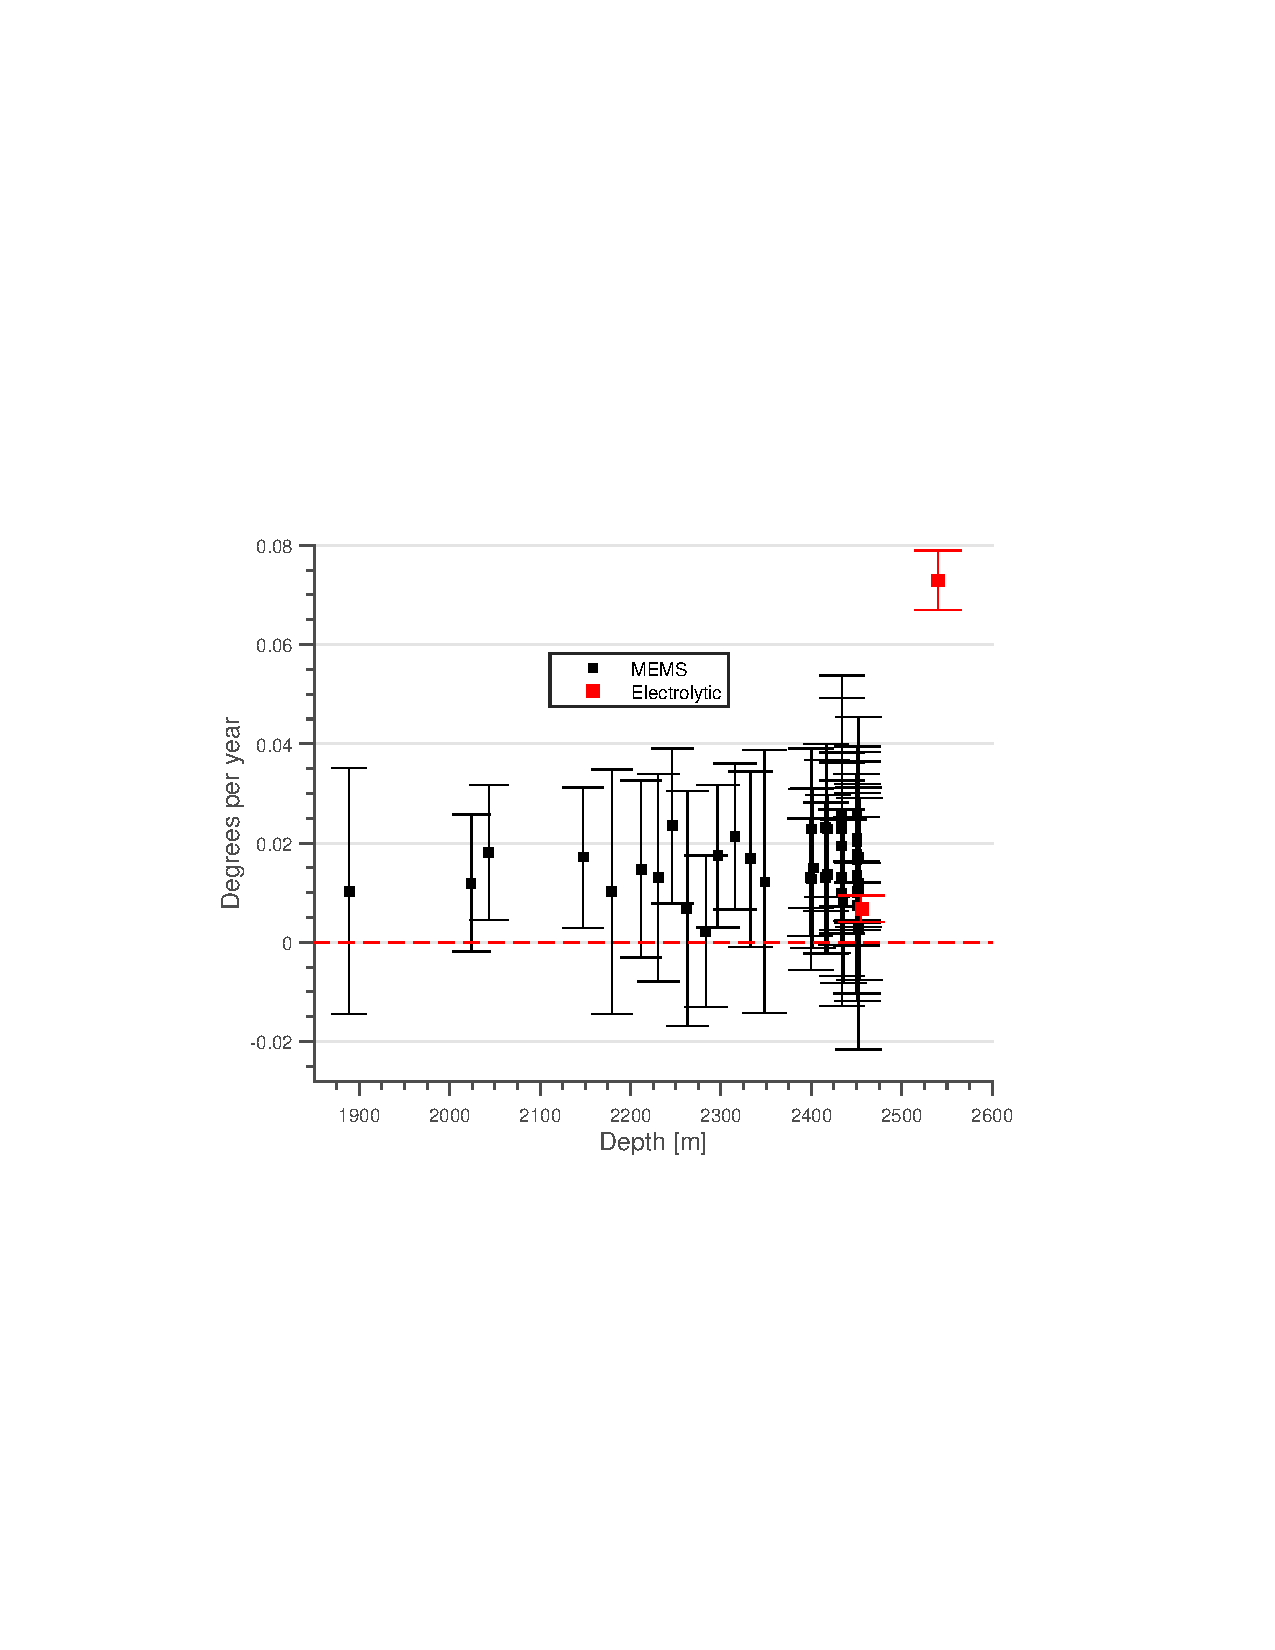
\includegraphics[width=0.7\textwidth]{graphics/tilt/tilt.pdf}
\caption{Long term average inclination readings from two electrolytic (red) and 42 MEMS (black) tilt sensors installed in 2007-2011.  Error bars show deviation from the average trend.  The reading at \unit[2540]m indicates increasing strain below the IceCube instrumented volume.}
\label{fig:tilt}
\end{figure}


In most glaciers at sufficiently great depth, ice strain undergoes a transition from compression-dominated to shear-dominated with small-scale folding \cite{montagnat14,jansen16}.  This transition depth depends on temperature \cite{price2002temperature}, grain size, and impurities, and is associated with a strong single maximum polycrystalline ice fabric \cite{cuffey10}.  The deep sensor at \unit[2540]m has shown a persistent \numrange[range-phrase = --]{0.07}{0.08} degrees of tilt per year since installation (shear 0.0013 per year).  Tilt sensors within the IceCube instrumented volume, at depths \SI{<2450}m,  show essentially no movement.  Although the MEMS chips have less reliable long-term stability and higher noise than the electrolytic inclinometers, the MEMS readings are consistent with $\lesssim$\unit[0.01]degrees of tilt per year with no apparent depth dependence.  Profiles of the atmospheric dust embedded in the ice \cite{I3:dustlogger} show no indication of folding and appear undisturbed over the full IceCube depth.
  
